\section{Structure Determination of NeAr Clusters}

In general, the structure determination of heteronuclear noble gas
clusters is an unsolved problem. However, the maximization of the cohesive
energy suggests a core of argon atoms surrounded by neon atoms.
Electron-electron coincidence experiments proved their existence by the
presence ICD electron from NeAr-ICD processes \cite{Lundwall07}.

The clusters consist of neon and argon atoms. Since an inner-valence vacancy in
the Ne2s can decay both via NeNe-ICD and NeAr-ICD, both competing processes
are expected to be observed in an experiment. In the literature most
investigations focussed on the NeAr-ICD, because it, until recently, was not
possible to measure the NeNe-ICD as well \cite{Fasshauer14_1}.
From these studies, large NeAr clusters established by coexpansion and
consisting of an argon core with
approximately 1000 atoms were determined to have a core-shell structure
\cite{Lundwall07,Barth_diss}
and to have a temperature of \unit[40 -- 50]{K} \cite{Barth_diss}.
In his PhD thesis, Barth suggested the possibility to gain information about
the cluster structure from the efficiency of the NeAr-ICD compared to the
total decay of the Ne2s ionization. This was proposed to be possible, since
the sum over the NeNe-ICD and NeAr-ICD previously had been shown to
cause almost the total decay of the Ne2s vacancy \cite{Marburger_diss}.
The results indicated an increasing NeAr-ICD efficiency with increasing
cluster size and hence a smaller surface-to-bulk ratio.

This structure determination, as is going to be shown, is indeed possible
because the decay widths of the competing NeNe-ICD and NeAr-ICD processes
are of the same order
of magnitude and therefore both signals are observable. Additionally, as shown
in the preceeding section about ArXe clusters, the secondary electron spectrum
crucially depends on the underlying structure.

Recently, the NeNe-ICD in NeAr clusters could be measured. Therefore, I will
present the structure determination of NeAr clusters from ICD electron
spectra by comparison of experimental spectra with theoretical calculations.

The chapter is structured as follows: First, the experimental results are
presented and the computational details for the simulation of the ICD
electron spectra are demonstrated. Afterwards, the manifold of different 
hypothetical cluster structures are introduced. Finally, the comparison
between the experimental findings and theoretical predictions will be used
for the determination of mean cluster structures.


\subsection{Experimental Results}
Recently, it was possible to measure the full secondary electron spectrum
of NeAr clusters under different experimental conditions as shown in Figure
\ref{figure:NeAr_exp_spectrum} and Table \ref{table:expansion_conditions}.

\begin{figure}[h]
  \centering
  \includegraphics[scale=1.7]{pics/exp_near_coinc_sets.eps}
  \caption{Electron-electron coincidence spectra for NeAr clusters
           showing both NeNe-ICD and NeAr-ICD signals \cite{Fasshauer14_1}.}
  \label{figure:NeAr_exp_spectrum}
\end{figure}

\begin{table}[!h]
 \centering
 \caption{Assignment and expansion parameters of the five different
          cluster ensembles. Included are also the resulting mean
          cluster sizes calculated for the homogeneous species according
          to the formalism intruduced by Hagena \it{et al.}
          \cite{Hagena72}}
  \begin{tabular}{c c c c c c}
          \toprule
           designation    &       Ar content in   & expansion & nozzle & $\langle N\rangle _{Ne}$ & $\langle N\rangle _{Ar}$ \\
                                          &       initial mixture &  pressure & temperature & &  \\
          \midrule
          Set 1   &       \unit[1.7]{\%}  &       \unit[0.26]{bar}        &       \unit[63]{K}    &       \unit[5]        &       \unit[520]      \\
          Set 2   &       \unit[7.4]{\%}  &       \unit[0.40]{bar}        &       \unit[60]{K}    &       \unit[17]       &       \unit[1850] \\
          Set 3   &       \unit[1.7]{\%}  &       \unit[0.25]{bar}        &       \unit[57]{K}    &       \unit[7]        &       \unit[810]  \\
          Set 4   &       \unit[7.4]{\%}  &       \unit[0.24]{bar}        &       \unit[58]{K}    &       \unit[6]        &       \unit[670]  \\
          Set 5   &       \unit[1.0]{\%}  &       \unit[0.16]{bar}        &       \unit[54]{K}    &       \unit[3]        &       \unit[380]  \\
          \bottomrule
  \end{tabular}
\label{table:expansion_conditions}
\end{table}

The spectra have been normalized to the peak height of the NeAr-ICD signal.
It can clearly be seen that for different experimental conditions the
size of the NeNe-ICD peak varies compared to the NeAr-ICD peak as explicitely
listed in Table \ref{table:clustervalues}. This can be
explained both by different cluster sizes and by different cluster structures
as I am going to show in this thesis. Both the main NeNe-ICD and the NeAr-ICD peak
have a shoulder at higher energies. For NeAr dimers such a structure has
been proposed to potentially stem from vibrations. However, such bound vibrational
states above the ground state do not exist in neon dimers. I am going to show
that this peak structure can be related to \ac{ICD} processes with next nearest
neighbours. Still, excitations to higher vibrational states might contribute
to the peak structure as well.

\begin{table}[!h]                                                                                                                                       
 \centering                                                                                                                                      
 \caption{Experimental results. Percentaged values are contributions to the
          respective total values. The cluster band onsets are given
          at half the peak height of the respective feature.}
   \begin{tabular}{c c c c c}                                                                                                              
           \toprule
            designation    &       Ar content in   & onset Ar3p                    & onset Ne2p            & Ne-Ar ICD     \\
                                           &       final cluster   &   cluster band                & cluster band          & contribution  \\
           \midrule
           Set 1   &       \unit[47 $\pm$ 10]{\%}  &       \unit[14.7$\pm$ 0.1]{eV}        &       \unit[20.93$\pm$ 0.08]{eV}      &       \unit[63 $\pm$ 7]{\%}   \\
           Set 2   &       \unit[35 $\pm$ 5]{\%}   &       \unit[14.6$\pm$ 0.1]{eV}        &       \unit[20.86$\pm$ 0.08]{eV}      &       \unit[61 $\pm$ 10]{\%}  \\
           Set 3   &       \unit[21 $\pm$ 4]{\%}   &       \unit[14.8$\pm$ 0.1]{eV}        &       \unit[20.86$\pm$ 0.08]{eV}      &       \unit[38 $\pm$ 5]{\%}    \\
           Set 4   &       \unit[20 $\pm$ 4]{\%}   &       \unit[14.8$\pm$ 0.1]{eV}        &       \unit[20.86$\pm$ 0.08]{eV}      &       \unit[53 $\pm$ 6]{\%}    \\
           Set 5   &       \unit[8 $\pm$ 2]{\%}    &       \unit[15.0$\pm$ 0.1]{eV}        &       \unit[20.89$\pm$ 0.08]{eV}      &       \unit[28 $\pm$ 3]{\%}    \\
           \bottomrule
   \end{tabular}
\label{table:clustervalues}                                    
\end{table}




\subsection{Computational Details}
The energies of the secondary electron were calculated using the
experimentally obtained ionization energies given in Table \ref{exp_input}.

\begin{table}[h]
 \caption{Experimental values used for the estimation of the decay widths
          \cite{Fasshauer14_1}.}
 \label{exp_input}
 \centering
 \begin{tabular}{lc}
  \toprule
  indicator            &  value \\
  \midrule
  SIP(Ne2s)            &  \unit[47.75]{eV} \\
  SIP(Ne2p)            &  \unit[21.10]{eV} \\
  SIP(Ar3p)$_{c<3}$    &  \unit[15.40]{eV} \\
  SIP(Ar3p)$_{c\ge 3}$ &  \unit[15.20]{eV} \\
  \bottomrule
 \end{tabular}
\end{table}

The distance dependence of the NeAr dimer was non-relativistically calculated with
the Fano-Stieltjes procedure implemented in Dirac \cite{DIRAC13,Fasshauer14_2}
with an aug-cc-pV6Z basis set on both atoms. 
Additional basis functions of five $s$, $p$ and $d$ functions each of the
KBJ type \cite{Kaufmann89} were introduced on a ghost atom in the
geometric center of the dimer.

Since inversion symmetry is until now not treated correctly,
for the neon dimer decay width data from the literature is used, which was
obtained with the same method and a comparable basis set \cite{Averbukh06_1}.
The resulting decay widths are shown in Figure \ref{figure:fitted_NeAr_widths}
and the corresponding lifetimes are in Table \ref{table:NeAr_gammas} compared
to other values from the literature.

\begin{table}[htb]
 \centering
 \caption{Decay widths of the NeNe-ICD and NeAr-ICD obtained
          using different theoretical
          methods and from experiment.}
 \begin{tabular}{lcrcrcr}
  \toprule
        & \multicolumn{2}{c}{Theory used} & \multicolumn{2}{c}{Theory Comp.} & \multicolumn{2}{c}{Experiment} \\
  \midrule
   NeNe & \unit[60.4]{fs} & \cite{Averbukh06_1} & \unit[92]{fs} & \cite{Vaval07} & \unit[$150\pm 50$]{fs} & \cite{Schnorr13}\\
   NeAr & \unit[44.2]{fs} & This work & \unit[36]{fs} & \cite{Scheit06} &  --  &\\
  \bottomrule
 \end{tabular}
 \label{table:NeAr_gammas}
\end{table}

The NeAr-ICD has a higher decay width than the NeNe-ICD, but since the
actual value of the decay width strongly depends on the method and basis set
used for its description, larger discrepancies are normal. For the decay
width estimation of the NeAr clusters the values of the first column were
chosen, because they were both calculated using the FanoADC Stieltjes approach
with comparable basis set size.

\begin{figure}[h]
 \centering
 \begin{tikzpicture}[scale=1.5]

\begin{loglogaxis}[%scale=1.5,
             domain=2:30,
             %y domain=1E-8:10,
             restrict expr to domain={y}{1E-8:15},
             xlabel={Beschriftung x},
             xtick={2,4,...,10,15,...,25},
             xticklabels={2,4,6,8,10,15,20,25},
             ylabel={Beschriftung y},
             title={Titel}
             ]

\addplot[only marks,
         mark=x,
         thick,
         diplom4
        ]
        table[
        x expr = \thisrowno{0},
        y expr = \thisrowno{1}
        ]
        {../data/NeAr.dat};
        \addlegendentry{NeAr data};
	
\addplot[
        very thick,
        diplom3,
        samples=200
	]
	{1211057096516.005371 * exp(-11.074016*x) + 23.797274/x^6};
        \addlegendentry{NeAr fit};

\addplot[only marks,
         mark=x,
         thick,
         diplom2
        ]
        table[
        x expr = \thisrowno{0},
        y expr = \thisrowno{1}
        ]
        {../data/Ne2.dat};
        \addlegendentry{Ne$_2$ data};
	
\addplot[
        very thick,
        diplom1
	]
	{19.643762 * exp(-2.789916*x) + 6.204031/x^6};
        \addlegendentry{Ne$_2$ fit};

		
\end{loglogaxis}
\end{tikzpicture}

 \caption{Decay widths of the NeNe-ICD and NeAr-ICD processes fitted to
          curves for the decay width estimation of the NeAr clusters.}
 \label{figure:fitted_NeAr_widths}
\end{figure}

For each structure defined in the following section the NeNe-ICD and NeAr-ICD
spectra were calculated using the programme HARDRoC \cite{HARDRoC}.




\subsection{Hypothetical, idealized structures of the NeAr clusters}

It is known that small noble gas clusters preferably form icosahedral structures,
while with increasing cluster size a fcc structure becomes more favorable. This transition
occurs at cluster sizes in the range from 750 to 3500 atoms \cite{Martin96,Doye97,Hartke02}.
For the simulations it is assumed that the clusters of all
five experimental cluster sets have 
icosahedral structure. For all sets but set 2 the expansion conditions should result in clusters 
with mean sizes below 750 (see Table \ref{table:expansion_conditions}). Still,
the mean size of the clusters of set 2 is well below 3500.

\begin{figure}[!ht]
 \centering
 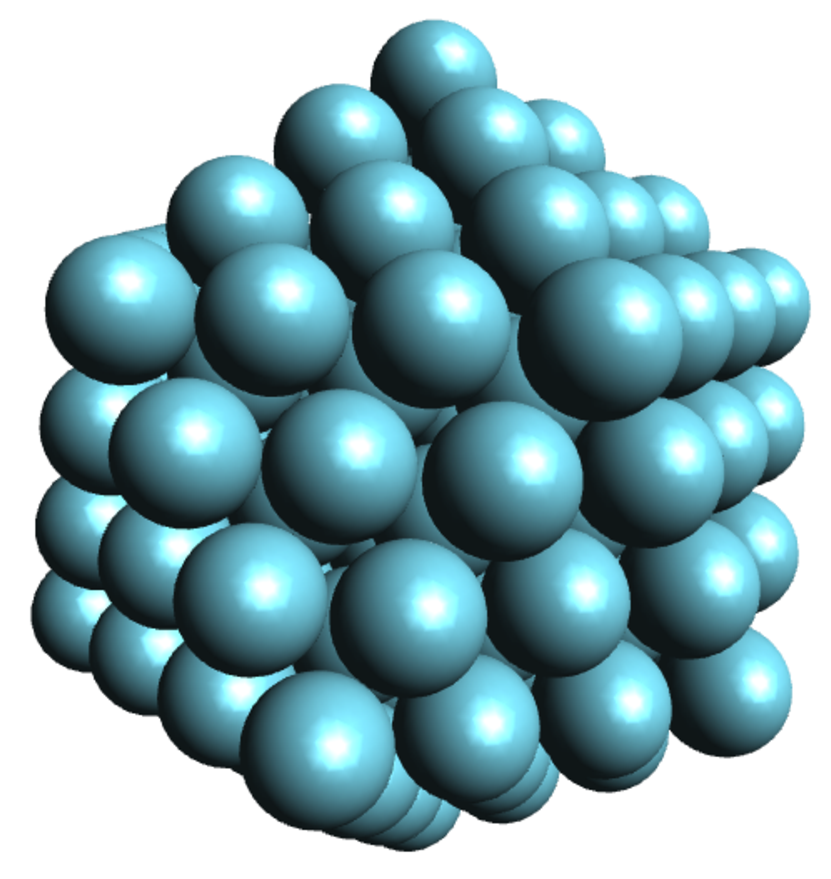
\includegraphics[scale=0.5]{pics/Ar_pure.eps}                        
 \caption{An icosahedral argon cluster with an edge consisting of 
          $c=\unit[4]{atoms}$, containing \unit[147]{atoms},
          distributed over four shells. \unit[55]{atoms} belong
          to the core, 12 are at the vertices, 60 in the edges and 20 inside the
          surfaces.}
 \label{figure:Ar_pure}
\end{figure}    

The actual cluster formation process is understood as follows. First, a three particle
collision has to take place to form argon dimers. Subsequently, single atoms are added to the dimer 
due to collisions. At a later stage these clusters can also collide to form larger clusters. This process,
called coagulation, becomes the dominant process for the formation of very large clusters. 
The experiment of Lundwall et al. \cite{Lundwall07} was interpreted to
show clusters consisting of an argon core with distinct, complete neon
shells around it, which is plausible, since according to the sum of van der Waals
energies, this should be the most stable kind of clusters.
Therefore this structure is chosen as a starting point for the considerations
about the average structure of the clusters.

In all structures considered throughout this thesis the core is build as
 an icosahedral
structure of argon atoms as shown in Figure \ref{figure:Ar_pure}.
In this example, it has an edge length
of $c=\unit[4]{atoms}$ and consists of $n_{Ar}=\unit[147]{atoms}$, which can be
calculated as \cite{Martin96}

\begin{equation}
  n_{atoms} = \frac{10}{3} c^3 - 5 c^2 + \frac{11}{3} c -1 .
\end{equation}

For the construction of the structure the minimum
distance between two argon
atoms is assumed to be twice the van der Waals
radius of argon $r_{Ar}=$ \unit[1.88]{\AA} \cite{Bondi64}. In order to abide by this
minimum distance in the case of two atoms in a surface position in different
shells, the distance of two atoms in the edges is slightly increased.

As is going to be seen in the discussion, the outcome of the experiment
cannot completely be explained by an argon core surrounded by complete neon shells.
This leads to considerations of other structures with an argon core somehow surrounded
by neon atoms. These are divided into three types, so that, in total, four
different classes of cluster structures are studied as
shown in Figure \ref{figure:structures}:

\begin{enumerate}
 \item complete shells
 \item incomplete shells around complete shells
 \item caps
 \item randomly arranged neon atoms around complete shells
\end{enumerate}

\begin{figure}[h!]
 \centering
 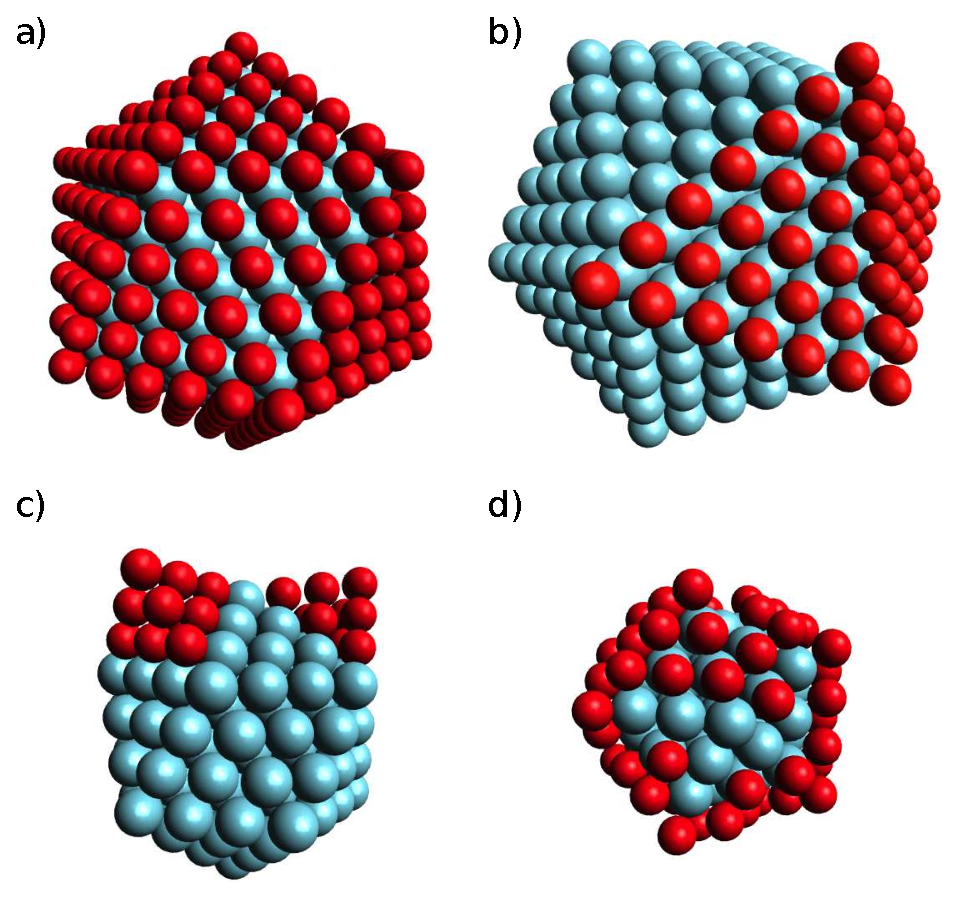
\includegraphics[scale=0.9]{pics/NeAr_structures1.eps}
 \caption{Structure classes considered in our calculations.\\
          a) complete shells, in this example $c=\unit[5]{atoms}$ with one layer
          neon atoms,\\
          b) incomplete shells, in this example
          $c=\unit[6]{atoms}$ with two covered trinangular surfaces
          of neon,\\
          c) caps, in this example $c=\unit[4]{atoms}$ with two caps,\\
          d) randomly arranged neon atoms around a full shell cluster,
          here $c=\unit[3]{atoms}$ directly covered by neon atoms
          with an argon content of \unit[47]{\%}.}
 \label{figure:structures}
\end{figure}

In the case of an argon cluster with one or more complete shells of neon
atoms around it, first the core structure is created and afterwards the
outer shells are constructed around it, such that the minimum distance between a
neon atom in the surface and an argon atom in the shell beneath is the sum
over the van der Waals radii, where $r_{Ne}=$\unit[1.54]{\AA} \cite{Bondi64}
(see Figure \ref{figure:structures} panel a).

Not all experimentally determined argon contents in the mixed clusters
fit to complete neon shells. Maintaining the idea of shells,
the possibility of incomplete shells is considered.
The cluster structures are created analogously to the
complete shells except that not all triangular surfaces areas of the argon core
are covered by neon atoms (for an example see Figure \ref{figure:structures}
panel b).

Another possibility is caps covering surface areas as shown
in Figure \ref{figure:structures} panel c. These structural elements
do not lead to minimum energies for clusters, but they might explain a
large number of neon-neon interactions compared to the number of
neon-argon interactions in the experiments.
The neon-neon distances within the caps are
calculated in the same
manner as described before for the (in-)complete shells.
A whole manifold of different positionings of several caps are in principle
possible, but calculations showed, that these different
placements of caps did not change the ratios of NeAr- to NeNe-ICD for a
constant number of caps. Since these structures cannot be distinguished
by ICD spectra, the
discussion is limited to structures containing different numbers of caps.

One could also think about neon atoms randomly arranged around a homonuclear
or heteronuclear cluster with complete shells and randomly attached neon
atoms around it as shown in Figure \ref{figure:structures} panel d.
It is constructed as a cluster with complete shells and afterwards adding
neon atoms in random positions of the next layer until the requested
$n_{Ar}/n_{Ne}$ ratio is reached.

All these structures are idealized and highly symmetric, which reduces
the computational cost. They were constructed using the set of \verb|icoclus|
scripts written for this purpose and explained in the
appendix \ref{section:icoclus}.
Vibrations inside the clusters will change the interatomic
distances and hence both the kinetic energies of the ICD electrons as well as
the decay widths. As has been shown for NeAr \cite{Scheit06}, the ICD processes
are faster than dynamical rearrangements, caused by Coulombic attraction
after the initiating ionization, or vibrations. In case of the neon dimer, the
ICD lifetime is of comparable size to the rearrangement time and hence
influences the ICD electron spectra \cite{Scheit03}. However, in clusters, the
initially ionized atom interacts with more than one other atom, which leads
to more neighbours it can undergo ICD with. Hence, the decay width increases
to first approximation linearly with the number of nearest neighbours.
At the same time, the larger number of neighbours stabilizes the position
of the initially ionized atom in space compared to the dimer.
Therefore, it is assumed that the structures given above are good
approximations to the decaying clusters.




\subsection{Interpretation of the graphs}

In order to have comparable numbers, for the theoretical estimations and
experimental results the entities chosen for the characterization of each
cluster structure and measurement are
the argon content in the cluster and the amount of
NeAr-ICD compared to the total ICD
$\frac{\Gamma_{NeAr}}{\Gamma_{NeAr}+\Gamma_{NeNe}}$.
Throughout the thesis, the same 
colour coding as for the experimental spectra
shown in Figure \ref{figure:NeAr_exp_spectrum} is used,
for which the numbers are listed in Table \ref{table:clustervalues}.
The results are going to be plotted as in Figure \ref{figure:incompl01_02_explain}.
As an example, the results for clusters of the class of an
incompletely filled neon shell
around an argon core with a an edge size of $c=2$
surrounded by one complete shell of neon atoms are shown.
Here, the ratio of NeAr-ICD to total ICD is plotted against the argon content
of the cluster. The results of the five different experimental conditions and their
errors are shown by the coloured areas, where the colour corresponds to the
set with the same colour as in Figure \ref{figure:NeAr_exp_spectrum}.
Additionally plotted are the theoretical results for the different structures
parted into first the classes of the structures and secondly by the size of the argon core.
The higher the argon content is, the less of the 20 surfaces of the underlying
complete shell is covered by either layer(s) or caps. The easiest way to interpret
the graphs is to start from a complete shell and then covering one surface. This
corresponds to the rightmost theoretical value within a group. Each step further
to the left refers then to one more covered layer with either caps or layers.\\

\begin{figure}[!h]
  \centering
  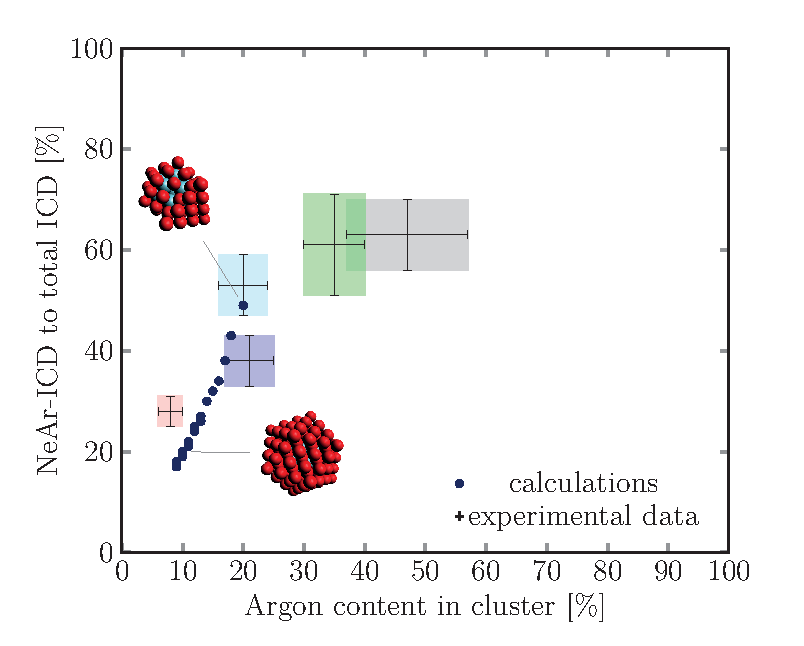
\includegraphics[scale=0.75]{pics/incompl01_02_mit_inlays.eps}
  \caption{NeAr-ICD to total ICD ratio plotted against the argon content
           in the cluster for both experimental results for all five sets of
           conditions as well as theoretical calculations for cluster structures
           with an incomplete outermost shell surrounding an argon core of
           $c=2$ and one additional complete neon shell. For illustrative purposes,
           pictures of two structures are included at their respective
           theoretical values.}
  \label{figure:incompl01_02_explain}
\end{figure}

By looking for agreements of theoretical and experimental values
possible structures are deduced.
The agreements between experimental and theoretical results are evaluated
using the graphical distance from the experimental results
\begin{equation}
  d = \sqrt{\Delta_{Ar}^2 + \Delta_{\Gamma}^2}    ,
\end{equation}
where $\Delta_{Ar}$ and $\Delta_{\Gamma}$ denote the deviation of the argon content
and the ratio of NeAr-ICD decay width and the total decay width, respectively.
Only such structures are considered, where the argon content of the model
structure lies within the error range of the experimental findings.


\subsection{Assignment of the different measurements to cluster structures}
For the assignments the following criteria are used:

\begin{itemize}
 \item onsets of single ionization potentials for the determination
       of the size of the argon core
 \item positions of NeAr-ICD peak
 \item relative expected mean cluster sizes
       (see Table \ref{table:expansion_conditions})
 \item agreement of predicted and measured ICD (see Table \ref{table:assignments})
\end{itemize}

From the onsets of the single ionization potentials and the position of the
NeAr-ICD peak at a lower energy it is deduced that the mean argon core of set 5
is the smallest of all measured ensembles. Since the nearest neighbours have
the largest influence of such a shift these clusters can be interpreted to have
an edge length of either $c=1$ or $c=2$.\\
Since the estimations of mean cluster sizes based on Hagena refer to expansions
of only one atom type, only the results with the same argon content should
be compared. From this the core of set 2 can be expected to be bigger than the core
of set 4 and the core of set 3 can be expected to be slightly larger
than the core of set 1.
These estimations do not have to resemble the final conclusions, since the
approach is only valid for homogeneous clusters, but can give hints
in the following procedure. The assignment due to geometrical distance
of the predicted results from the experimental counterparts is to be found in
Table \ref{table:assignments}. There, the best results for all sets are shown
in the following way: $c$ depicts the number of atoms in the longest edge
of the argon core, which is then covered by a number of additional complete
neon shells with additional covered triangular surfaces or randomly arranged atoms
and $d$ denotes the geometrical distance.

\begin{table}[!h]
  \caption{The smallest geometric distances for each set of clusters
           and the corresponding cluster structures.
           Note that for set 4 only the random arrangement is listed,
           for which the argon content exactly equals the experimental one.}
  \centering
  \begin{tabular}{lccccc}
    \toprule
     Set  & $c$ & complete Ne shells & covered surfaces & random & $d$\\
    \midrule
      1   & 4   &          1         &        1         &   -    & 2.000\\
      1   & 5   &          1         &        2         &   -    & 4.472\\
      1   & 2   &          0         &        5         &   -    & 4.472\\
    \midrule
      2   & 3   &          1         &        -         &   x    & 1.000\\
      2   & 3   &          1         &        1         &   -    & 3.162\\
      2   & 2   &          0         &        8         &   -    & 4.123\\
    \midrule
      3   & 2   &          1         &        3         &   -    & 4.000\\
      3   & 3   &          1         &        7         &   -    & 4.123\\
      3   & 3   &          1         &        8         &   -    & 4.472\\
    \midrule
      4   & 2   &          1         &        -         &   x    & 2.000\\
      4   & 2   &          1         &        1         &   -    & 4.000\\
    \midrule
      5   & 2   &          1         &       13         &   -    & 8.246\\
      5   & 2   &          1         &       14         &   -    & 9.220\\
      5   & 2   &          1         &       15         &   -    & 9.220\\
    \bottomrule
  \end{tabular}
  \label{table:assignments}
\end{table}

The structure assignment is going to be discussed in descending order
of the set number, which more or less corresponds to a discussion with
increasing size of the clusters.\\
The assignment is started with set 5 (red). As already mentioned,
these clusters can be expected
to be small and, additionally, the smallest ones measured. These expectations are
in agreement with the results of Figure \ref{figure:incompl01_02_explain}
(also to be found in the
appendix in Figure \ref{incompl01-core02}), where the red square
can be matched with a cluster to an argon core with $c=2$, one complete
shell of neon atoms 
and one almost complete
shell with 13 -- 20 out of 20 surfaces covered by neon atoms. None of the
theoretical estimates coincide with the experimental findings. This might be
explained by even smaller clusters not showing an icosahedral argon core, but
a coagulation of 2--11 atoms plus some neon atoms.

Set 4 (turquoise) shows a very good agreement for a structure with $c=2$ with one
complete shell of neon atoms and some additional atoms (see Figures
\ref{random-core02} and \ref{incompl01-core02} or in the example above).
Whether these atoms are
randomly arranged around the complete shells or are to be found together cannot
finally be decided. From the geometric distance, the random arrangement should
be preferred.

The results of set 3 (blue) shows a good agreement with structures
of $c=2$ or $c=3$ surrounded by one complete shell of neon atoms and additional
neon atoms covering 3 or 7 -- 8 triangular surfaces, respectively 
as shown in Figures \ref{incompl01-core02} and \ref{incompl01-core03}. 

With the two latter assignments it is possible to distinguish
the structures of two cluster manifolds with the same argon content by utilizing the
ICD spectra.

Set 2 (green) can be assigned to core sizes of $c=2-3$ plus further neon atoms
(see Figures \ref{incompl00-core02} and \ref{incompl01-core03}).
In the case of $c=3$, one additional complete shell of neon atoms fits
best to the experimental results, but as for set 4 the arrangement as such for
some few additional atoms can either be random or coagulated.
In case of $c=2$ the best fit holds for no additional complete shell of
neon atoms but with 8 triangular surfaces covered, the shell is almost halfway filled.
Further structures with larger core sizes as $c=4$
are also quite probable. Considering, that 
both from Hagena's approach and the single ionization potential
onsets of the Ar3p band, set 2 is supposed to have the largest mean structure
core, the latter structures might be closer to reality than the ones of the small clusters
with $c=2,3$.

Due to the large error bars, set 1 (black) can be assigned to a whole manifold
of different structures with $c = 2 - 6$ within the error bars
either with caps or, more probably,
with about one complete shell of neon atoms, plus maybe additional covered surfaces
or randomly surrounded by neon atoms. Since caps should be energetically less
favourable than the other structures, I will suspend those structures
and concentrate
on the rest.
From Hagena's approach I concluded that the core of the clusters of set 1
should be slightly
smaller or of comparable size as the clusters from set 3. Therefore I assume
the average cluster structure to consist of an argon core of $c=2-4$ shells
with one complete neon shell and possibly one further incomplete shell, of
which I cannot give more detailed information.

One might have to consider completely different structures not investigated in this
thesis. Formed, mixed clusters might collide and coagulate, yielding
structures impossible to be estimated by a core-shell structure of the kinds
presented in this work. 

From the best agreement of the calculated NeAr-ICD to total ICD ratios listed in Table
\ref{table:assignments}, the corresponding estimated spectra are folded
with gaussians with a width of \unit[250]{meV}
and are plotted in Figure
\ref{figure:theo_specs}.
From these spectra and the underlying calculations
I conclude, that the shoulders of both the NeNe-ICD and the NeAr-ICD peak
at \unit[2.5--4]{eV} and \unit[8--10]{eV}
correspond to next-nearest neighbours inside the clusters, while the differences
in the main peak stem from almost equal interatomic distances but different positions
in the cluster such as corner, edge or surface.\\
The main peaks of the NeNe-ICD correspond well with the experimental observations
of Figure \ref{figure:NeAr_exp_spectrum}.\\
The onset of the NeAr-ICD peak depends on the shielding of the argon atom
and hence the cluster size. For set 5 the assignment seems to be correct, while
for set 4, the experiment shows a higher energy of the ICD electron. 
This deviation implies that either the core of the mean cluster structure
is larger than evaluated from the theoretical calculations or that
the choice of $c=3$ as the minimum core size for the for the lower ionization
potential of the Ar3p was wrong.
The truth, however, is not a spontaneous jump from one shell to the other, but rather a decrease
with more and more atoms. If one is interested in clusters of $c\le2$ only, one
should take care of a more detailed description of the different ionization
potentials for different cluster sites.

\begin{figure}[!ht]
  \centering
      \begin{tikzpicture}

        \begin{axis}[
            use units,
            x unit=eV,
            y unit=a.u.,
%            title={Spektrum},
            xmin=0,
            xmax=10.5,
            axis x line=bottom,
%            axis x discontinuity=parallel,
            ymin=0,
            ymax=3.4,
            axis y line=left,
            samples=1000,
            scale=1.00,
            legend style={draw=none},
            legend cell align=center,
            legend pos=outer north east
            ]

        \addplot[
            mark=none,
            color=black,
            ]
            table[
            x expr=\thisrowno{0},
            y expr=\thisrowno{1} * 25.4518
            ]
            {data/near_clusters/set1.sp};
        \addplot[
            mark=none,
            color=green,
            ]
            table[
            x expr=\thisrowno{0},
            y expr=\thisrowno{1} * 27.0625
            ]
           {data/near_clusters/set2.sp};

        \addplot[
            mark=none,
            color=blue,
            ]
            table[
            x expr=\thisrowno{0},
            y expr=\thisrowno{1} * 43.2460
            ]
            {data/near_clusters/set3.sp};

        \addplot[
            mark=none,
            color=cyan,
            ]
            table[
            x expr=\thisrowno{0},
            y expr=\thisrowno{1} * 35.4689
            ]
            {data/near_clusters/set4.sp};

        \addplot[
            mark=none,
            color=red,
            ]
            table[
            x expr=\thisrowno{0},
            y expr=\thisrowno{1} * 76.3945
            ]
            {data/near_clusters/set5.sp};
        \end{axis}
    \end{tikzpicture}


  \caption{Calculated ICD electron spectra for those structures given in Table
           \ref{table:assignments} with the best agreement to the experimental
           argon content and NeAr-ICD to total ICD ratio. The intensities are given
           in arbitrary units and are normalized to the peak height of the NeAr-ICD
           peak and the spectra are folded by Gaussians with widths of \unit[250]{meV}.
           The theoretically calculated specrta nicely match the experimental ones in Figure
           \ref{figure:NeAr_exp_spectrum}.
           Both, the NeNe-ICD peak at low energies and the NeAr-ICD peak
           at higher kinetic energies, show a peak structure which can be related
           to different distances of the atoms involved in the process within the
           clusters. For more details, see the text.}
  \label{figure:theo_specs}
\end{figure}

\subsection{Conclusions}
I have developed a method for the analysis of a mean cluster
structure of noble gases utilizing the relative ICD decay widths
of two competitive decay processes. This I have exploited onto
five different cluster ensembles. I am able to explain the
spectra by different underlying mean structures. From the results I conclude, that
clusters formed in a supersonic beam most likely can be described
by a core-shell structure with additional layers. In some limited cases,
when only few additional neon atoms around complete shells are needed
to fulfill the argon content, the random arrangement seems to be possible.\\
%It is to be investigated, whether this method opens a possible structure
%analysis for distiguishing an underlying icosahedral structure from a
%crystal like fcc one.
